\documentclass[
12pt,				  % Tamanho da fonte principal
openright,			  % Capítulos começam em pág ímpar (insere página vazia caso preciso)
oneside,			  % "oneside" (imprime no verso da folha) ou "twoside" (não imprime no verso da folha)
a4paper,			  % Tamanho do papel
chapter=TITLE,		  % Títulos de capítulos convertidos em letras maiúsculas
%section=TITLE,		  % Títulos de seções convertidos em letras maiúsculas
%subsection=TITLE,	  % Títulos de subseções convertidos em letras maiúsculas
%subsubsection=TITLE, % Títulos de subsubseções convertidos em letras maiúsculas
english,			  % Idioma adicional para hifenização
brazil				  % O último idioma é o principal do documento
]{abntex2}              % Usa a classe Abntex2

% ------------------------------------------------------------------------------------------------------------------------------
% Importando Pacotes
\usepackage{helvet}                          % Seleção da fonte Helvet
\usepackage[T1]{fontenc}		             % Seleção de códigos de fonte.
\usepackage[utf8]{inputenc}		             % Codificação do documento (conversão automática dos acentos)
\usepackage{hyperref}                        % Usado para modificar metadados do pdf
\usepackage{graphicx}                        % Inclusão de gráficos e gerenciar imagens
\usepackage{microtype} 			             % Para melhorias de justificação
\usepackage{mathtools}                       % Torna equações bonitas
\usepackage{listings}                        % Inserir algoritmos de programação
\usepackage{listingsutf8}                    % Inserir algoritmos de programação apresentando acentos
\usepackage{amsfonts}                        % Conjunto de fontes para uso em matemática, incluindo: símbolos matemáticos extras
\usepackage{color}				             % Controle das cores
\usepackage[brazilian,hyperpageref]{backref} % Páginas com as citações na bibliográficas
\usepackage[num]{abntex2cite}	             % Estilo de citações
\usepackage{indentfirst}                     % Identifica o primeiro parágrafo de cada seção.
\usepackage{mathrsfs}                        % Permite um novo estilo de letras
\usepackage{longtable}                       % Permite o uso de tabelas longas
%\usepackage{mathfont}                       % ??
% ------------------------------------------------------------------------------------------------------------------------------

% --------------------------------------------------------------------------------------------------------------------------------------------------------------------------------------------------------------
% Informações de dados para CAPA e FOLHA DE ROSTO
\titulo{TÍTULO DO TRABalho}
\newcommand{\subtitulo}{SUBTÍTulo (SE HOUVER)} % Cria um subtitulo
\newcommand{\imprimirSubtitulo}{\subtitulo}    % Insere subtitulo na capa
\autor{nome do autor}
\local{Patos de Minas}
\orientador{(Nome do Orientador)}
\data{2020}
\instituicao{ INSTITUIÇÃO  \par  Setor Subordinado à Instituição  \par }
\preambulo{Relatório Parcial apresentado como um dos requisitos de avaliação na disciplina Instalações Elétricas do Curso de Engenharia de Eletrônica e Telecomunicações da Universidade Federal de Uberlândia.}
% --------------------------------------------------------------------------------------------------------------------------------------------------------------------------------------------------------------

% ------------------------------------------------------------------------------------------------------------------------------------------------------------------
% Definições iniciais
\renewcommand{\familydefault}{\sfdefault}                                        % Altera a fonte principal para Helvet ("Arial")
\linespread{1.43}                                                                % Para espaçamento entre linhas Word 1.5
\setlength{\parindent}{1.5cm} % ??
\citebrackets[]                                                                  % Referências entre colchetes
\renewcommand{\rmdefault}{\sfdefault}                                            % ??
\renewcommand\ABNTEXchapterfontsize\Large                                        % Altera a fonte dos capítulos para 17 pt
\renewcommand{\ABNTEXchapterfont}{\sffamily\bfseries}                            % Altera a fonte dos capítulos para negrito
\renewcommand\ABNTEXsectionfontsize\large                                        % Altera a fonte das seções para 14 pt
\renewcommand{\ABNTEXsectionfont}{\sffamily\bfseries}                            % Altera a fonte das seções para negrito
\renewcommand\ABNTEXsubsectionfontsize\large                                     % Altera a fonte das subseções para 14 pt
\renewcommand{\ABNTEXsubsectionfont}{\sffamily\bfseries}                         % Altera a fonte das subseções para negrito
\definecolor{blue}{RGB}{41,5,195}                                                % Altera o aspecto da cor azul
\definecolor{codegreen}{rgb}{0,0.6,0}                                            % Cor para os algoritmos
\definecolor{codegray}{rgb}{0.5,0.5,0.5}                                         % Cor para os algoritmos
\definecolor{codepurple}{rgb}{0.58,0,0.82}                                       % Cor para os algoritmos
\definecolor{backcolour}{rgb}{0.99,0.99,0.99}                                    % Cor para os algoritmos
\renewcommand{\lstlistingname}{Algoritmo}                                        % Altera o nome no referenciação de algoritmos
\renewcommand{\lstlistlistingname}{Lista de algoritmos}                          % Altera o nome no referenciação de algoritmos
\lstset{numberbychapter=false}                                                   % Corrige a numeração dos algoritmos"
\newlistof{lstlistoflistings}{lol}{\lstlistlistingname}                          % Para remover “lstlistoflistings” do índice (toc)
\newcommand\ddfrac[2]{\displaystyle \frac{\displaystyle #1 }{ \displaystyle #2}} % Criando comando "\ddfrac{}{}" para frações matemáticas sempre com "\displaystyle"
%\mathfont{\sfdefault}                                                            % ??
\renewcommand{\backrefpagesname}{Citado na(s) página(s):~}                       % Configurações do pacote backref
\renewcommand{\backref}{}                                                        % Texto padrão antes do número das páginas
%
\renewcommand*{\backrefalt}[4]{                                                  % Define os textos da citação
	\ifcase #1 %
	Nenhuma citação no texto.%
	\or
	Citado na página #2.%
	\else
	Citado #1 vezes nas páginas #2.%
	\fi}%
%
\hypersetup{                               % Informações do PDF
	pdftitle={\@title},
	pdfauthor={Fábio Campos Ferreira},
	pdfkeywords={latex},
	pdfcreator={LaTeX},
	colorlinks=true,
	linkcolor=black,
	citecolor=black,
	urlcolor=black
}
\makeatletter
\setlength{\@fptop}{5pt} % Posiciona figuras e tabelas no topo da página quando adicionadas sozinhas
\makeatother
%
\makeatletter
\def\ScaleIfNeeded{                 % Criando comando "\ScaIfNeeded" para ajuste automático da escala das imagens
	\ifdim\Gin@nat@width>\linewidth
	\linewidth
	\else
	\Gin@nat@width
	\fi
}
\makeatother
\allowdisplaybreaks[1]
%
% ------------------------------------------------------------------------------------------------------------------------------------------------------------------



\begin{document}
\pretextual
\imprimircapa                         % Imprime a capa
%
\pdfbookmark[0]{\contentsname}{toc} % ??
\tableofcontents*                   % Insere sumario
\cleardoublepage                    % ??
% --------------------------------------------------------------------------------------------------------
% !TeX spellcheck = pt_BR
\chapter{Introdução a engenharia de micro-ondas}
\section{Ocupação do espectro eletromagnético}
\textbf{Espectro eletromagnético} é o conjunto de todas as frequências da energia eletromagnética.


As \textbf{bandas de frequências} ou \textbf{faixas} são subdivisões de frequências do espectro. A divisão é dada, pela Comitiva Internacional de Telecomunicações (CCIR),  pela relação
\begin{equation}
	0,3\times 10^N\leq f\leq 3\times 10^N
\end{equation}
onde\\
$f$ é a frequência;\\
$N$ é uma constante que caracteriza o grupo da divisão.

\section{As frequências de micro-ondas}

A \textbf{faixa de radiofrequência} (RF) apresenta limite superior de 300 MHz. Nesta faixa os sinais eletromagnéticos apresentam comprimentos de ondas muito curtos ($\lambda=1$ m).


A \textbf{faixa de micro-ondas} apresenta limite inferior de 300 MHz e superior de 300 GHZ ($\lambda=1\times 10^{-3}$ m), estando entre os sinais de RF e o infravermelho. Nesta faixa os sinais eletromagnéticos apresentam comprimentos de ondas ultra curtos.


Contudo, não é possível equipamento cobrirem toda esta faixa, então estes são projetados para operar em uma  determinada \textbf{faixa prática}. Estão foram definidas como\\
\begin{center}
	\begin{longtable}{cc}
		\textbf{Designação}&\textbf{Limites (GHz)}\\
		UHF&0,30 -3,00\\
		L &1,00 -1,55\\
		S &1,00 -3,95\\
		G &3,95 -5,85\\
		C &3,95 -8,20\\
		J &5,30 -8,20\\
		H &7,05 -10,0\\
		X &8,20 -12,4\\
		M &10,0 –15,0\\
		K$_{\text{U}}$ &12,4 -18,0\\
		K &18,0 -26,5\\
		K$_{\text{U}}$ &26,5 –40,0\\
		Q &23,0 -46,0\\
		U&40,0 -60,0\\
		V&40,0 -80,0\\
		E&60,0 -90,0\\
		W&58,0 –110\\
		F&90,0 –140\\
		N&80,0 –170\\
		D&110 -170\\
	\end{longtable}
\end{center}



As vantagens desta faixa são eficiência do processo de multiplexação,  grande diretividade das antenas, grandes larguras de faixas, confiabilidade do sistema, fácil instalação e custos compensados.

\section{Limitações dos elementos de circuitos em micro ondas}

Para um resistor real, a tensão $v$ é dada por
\begin{equation}
	v=iR
\end{equation}
onde\\
$R$ é a resistência nominal;
$i$ é a corrente.


Para um indutor real, a tensão $v$ é dada por
\begin{equation}
	v=L\ddfrac{di}{dt}
\end{equation}
onde\\
$L$ é a indutância nominal.


O indutor ainda apresenta uma reatância indutiva $X_L$ dada por
\begin{equation}
	X_L=\omega L=2\pi fL
\end{equation}
onde\\
$\omega$ é a frequência angular.	

Para um capacitor real, a tensão $v$ é dada por
\begin{equation}
	i=C\ddfrac{dv}{dt}
\end{equation}
onde\\
$C$ é a capacitância nominal.


O capacitor ainda apresenta uma reatância capacitiva $X_C$ dada por
\begin{equation}
	X_C=\ddfrac{1}{\omega C}=\ddfrac{1}{2\pi fC}
\end{equation}

\subsection{Resistor Real}

Para altas frequências, um resistor real pode ser representado como
\begin{center}
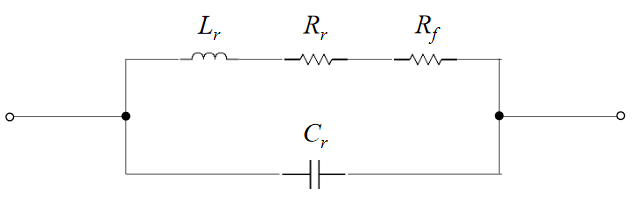
\includegraphics[width=\ScaleIfNeeded]{week01_ResumoResistorReal.png}
	\legend{Fonte: o autor.}
\end{center}
onde \\
$R_r$ é a resistência especifica;\\
$R_f$ é a resistência nos terminais;\\
$L_r$ é a indutância parasita dos terminais;\\
$C_r$ é a capacitância decorrente dos contatos metálicos com um meio dielétrico de separação.


A \textbf{condição de ressonância} ( quando aparte imaginaria da impedância assume valor zero) para o resistor real ocorre quando a frequência é igual a
\begin{equation}
f_{0res}=\ddfrac{\sqrt{1-R_t^2\left(\ddfrac{C_r}{L_r}\right)}}{2\pi\sqrt{L_rC_r}}
\end{equation}
onde\\
\begin{equation}
	R_t=R_r+R_f
\end{equation}
Esta relação é obtida encontrando a impedância equivalente do circuito, separando a parte imaginaria, igualando-a a zero e finalmente isolando a frequência.


A impedância se torna puramente resistiva, com valor dado por
\begin{equation}
R_{0res}=\ddfrac{R_t^2+\left(\omega_0L_r\right)^2}{R_t}=R_t\left(1+Q_r^2\right)
\end{equation}
onde\\
$\omega_0$ é a frequência angular na ressonância;\\
$Q_r$ é o fator de mérito do resistor na ressonância, dado por
\begin{equation}
Q_r=\ddfrac{\omega_0L_r}{R_t}
\end{equation}


\subsection{Indutor Real}

Para altas frequências, um indutor real pode ser representado como
\begin{center}
	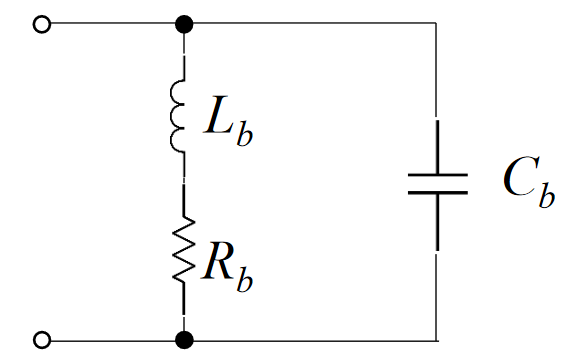
\includegraphics[height=7cm]{week01_ResumoIndutorReal.png}
	\legend{Fonte: o autor.}
\end{center}
onde \\
$L_b$ é a indutância especifica;\\
$R_b$ é a resistência devido à condutividade finita do material usado na construção do componente, aumentada pelo efeito pelicular e pelo efeito de aproximação das espiras;\\
$C_b$ é a capacitância distribuídas entre as espiras e entre suas extremidades.


A \textbf{condição de ressonância} para o resistor real ocorre quando a frequência é igual a
\begin{equation}
f_{0ind}=\ddfrac{\sqrt{1-R_b^2\left(\ddfrac{C_b}{L_b}\right)}}{2\pi\sqrt{L_bC_b}}
\end{equation}
Esta relação é obtida encontrando a impedância equivalente do circuito, separando a parte imaginaria, igualando-a a zero e finalmente isolando a frequência.


A impedância se torna puramente resistiva na ressonância, assumindo o valor
\begin{equation}
R_{0ind}=\ddfrac{R_b^2+\left(\omega_0L_b\right)^2}{R_b}=R_b\left(1+Q_b^2\right)
\end{equation}
onde\\
$Q_b$ é o fator de mérito do indutor na ressonância, dado por
\begin{equation}
Q_b=\ddfrac{\omega_0L_b}{R_b}
\end{equation}

\subsection{Capacitor Real}

Para altas frequências, um capacitor real pode ser representado como
\begin{center}
	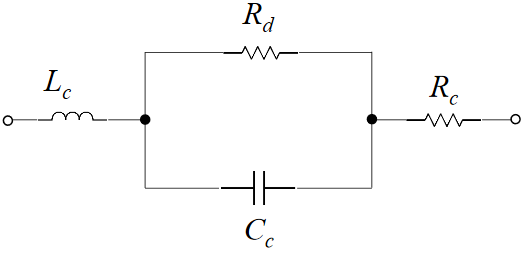
\includegraphics[height=7cm]{week01_ResumoCapacitorReal.png}
	\legend{Fonte: o autor.}
\end{center}
onde \\
$C_c$ é a capacitância especifica;\\
$R_d$ é a resistência de perdas no dielétrico;\\
$L_c$ é a indutância parasita associada aos terminas;\\
$R_c$ é a resistência parasita associada aos terminas.


A \textbf{condição de ressonância} para o resistor real ocorre quando a frequência é igual a
\begin{equation}
f_{0cap}=\ddfrac{\sqrt{1-G_d^2\left(\ddfrac{L_c}{C_c}\right)}}{2\pi\sqrt{L_cC_c}}
\end{equation}
onde\\
$G_d$ é dado por
\begin{equation}
G_d=\ddfrac{1}{R_d}
\end{equation}
Esta relação é obtida encontrando a impedância equivalente do circuito, separando a parte imaginaria, igualando-a a zero e finalmente isolando a frequência.


A impedância se torna puramente resistiva na ressonância, assumindo o valor
\begin{equation}
R_{0cap}=R_c+\ddfrac{R_d}{1+\left(\omega_0R_dC_c\right)^2}=R_c\left(1+Q_c^2\right)
\end{equation}
onde\\
$Q_c$ é o fator de mérito do capacitor na ressonância, dado por
\begin{equation}
Q_c=\ddfrac{\omega_0C_c}{G_d}
\end{equation}

%capitulo 2
\chapter{Ressonadores em micro-ondas}

\section{Cavidades Ressonantes}

Um \textbf{ressonador} é um dispositivo que exibe ressonância, ou seja, apresenta um fenômeno em que um sistema vibratório conduz outro sistema a oscilar com a maior amplitude em frequências especificas conhecidas como frequências ressonantes ou frequências naturais do sistema.


\textbf{Circuitos ressonantes} podem ser usados em filtros, osciladores, medidores de frequência e amplificadores sintonizados. Para baixas frequências, são construídos  apartir de resistores, capacitores e indutores. Para as frequências  de 30 MHz até 3 GHz são criados usando trechos de linhas de transmissão. Acima de 3 GHz, usa-se trechos de guias do ondas.


Uma \textbf{cavidade} pe um volume envolvido por uma superfície condutora, apresentando a possibilidade de excitação de um campo eletromagnético em seu interior.


Considerando a cavidade retangular abaixo
\begin{center}
	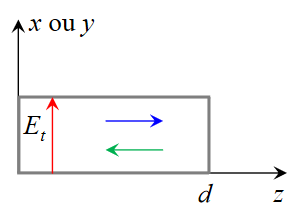
\includegraphics[height=7cm]{figCavidadeRetangular.png}
	\legend{Fonte: ver \cite{ribeiro}.}
\end{center}
esta, opera em modo TE$_{\text{mn}}$, ou seja, ??, com o campo elétrico da onda concentrado no plano transversal com eixo de propagação sendo \textbf{z} e limitada por $z=0$ e $z=d$.


O campo elétrico transversal é caraterizado por 
\begin{equation}
E_t=2A_i\mathsf{sen}\left(\ddfrac{p\pi z}{d}\right)\mathsf{sen}\left(\omega t\right)
\end{equation}
onde\\
$A_i$ é a amplitude do campo incidente;\\
$p$ é uma constante que indica o número de máximos de campo ( semi-períodos da senoide) na direção paralela ao eixo longitudinal;\\
$z$ é a posição sobre o eixo z;\\
$t$ é um instante de tempo.


Assim, o campo elétrico varia no tempo de forma senoidal no tempo e na distância longitudinal.


A frequência de ressonância de uma cavidade retangular é dado por
\begin{equation}
f_0=\ddfrac{c \sqrt{\left(\ddfrac{m\pi}{a}\right)^2+\left(\ddfrac{n\pi}{b}\right)^2+\left(\ddfrac{p\pi}{d}\right)^2}}{2\pi}
\end{equation}
onde\\
$m$ e $n$, assim como $p$, são os índices em modos TE e TM.


A frequência de corte de uma cavidade retangular é dado por
\begin{equation}
	f_c=\ddfrac{c \sqrt{\left(\ddfrac{m\pi}{a}\right)^2+\left(\ddfrac{n\pi}{b}\right)^2}}{2\pi}
\end{equation}

Um modo pode ser representado como TM$_{mnp}$/TE$_{mnp}$, onde os índices $m$, $n$ e $p$ assumem valores inteiros positivos e estão ligados diretamente com o período forma de onda do campo eletromagnético. O período dos componentes em função do eixo $x$ é determinada por $m$, eixo $y$ por $n$ e eixo $z$ por $p$, onde, a frequência de oscilação da onda no eixo será maior, quanto maior por o seu respectivo índice.
	

As dimensões de um guia ($a$,$b$ e $d$) normalmente apresentam a relação $a>d>b$. Critérios de proporcionalidade das dimensões foram propostos para reduzir as perdas de potência em frequências próximas de $f_0$, sendo elas
\begin{gather*}
a=\ddfrac{3c}{4f_0}\\
b=\ddfrac{3c}{8f_0}\\	
d=\ddfrac{3c}{2\sqrt{5}f_0}\\
\end{gather*}

%capitulo 2 aula 2

\section{Fator de mérito nas cavidades ressonantes}

O \textbf{fator de mérito} $Q_0$ é a razão entre a energia armazenada ($U_{máx}$) e dissipada ($P_d$).


A potência dissipada é a soma das dissipações no meio dentro da cavidade ($P_m$) e nas suas paredes ($P_c$). Então,
\begin{align*}
	Q_0&=\ddfrac{\omega_0U_{máx}}{P_d}\\
	Q_0&=\ddfrac{\omega_0U_{máx}}{P_m+P_c}\\
	Q_0&=\ddfrac{1}{\ddfrac{P_m}{\omega_0U_{máx}}+\ddfrac{P_c}{\omega_0U_{máx}}}\\
	Q_0&=\ddfrac{1}{\ddfrac{1}{Q_d}+\ddfrac{1}{Q_c}}\\
	Q_0&=\ddfrac{Q_cQ_d}{Q_c+Q_d}
\end{align*}
onde:\\
$\omega_0$ é a frequência angular de ressonância;\\
$Q_c$ é o fator
de mérito para a cavidade isolada;\\
$Q_d$ é o fator de mérito devido ao meio dentro da cavidade.


A energia máxima armazenada na frequência de ressonância é dada por 
\begin{equation}
	U_{máx}=\ddfrac{\varepsilon abd\eta^2H_0}{8}\left(\ddfrac{f_0}{f_c}^2\right)
\end{equation}
onde a impedância intrínseca do material dentro da cavidade ($\eta$) é definida como
\begin{equation}
	\eta=\sqrt{\ddfrac{i\omega_0\mu}{\sigma_d+i\omega_0\varepsilon}}
\end{equation}
onde:\\
$\mu$ é ??;\\
$\sigma_d$ é ??;\\
$\varepsilon$ é a permissividade dielétrica.


O fator de mérito devido o meio dentro da cavidade, também pode ser calculado por
\begin{equation*}
	Q_d=\ddfrac{\varepsilon'}{\varepsilon''}=\ddfrac{1}{\tan\left(\delta_d\right)}
\end{equation*}
onde:\\
$\varepsilon'$ é a parte real da permissividade dielétrica $\varepsilon$;\\
$\varepsilon''$ é a parte imaginaria da permissividade dielétrica $\varepsilon$;\\
$\delta_d$ é conhecido como fator ou tangente de perdas do meio.
	
	
O fator de mérito devido às perdas nas paredes apresenta cinco definições que dependem do modo eletromagnético e dos valores de $m$, $n$ e $p$. Para os modos TE$_{m0p}$
\begin{equation*}	Q_{c_{TEm0p}}=\left(\ddfrac{\lambda_0}{\delta_c}\right)\left(\ddfrac{abd}{2}\right)\left[\ddfrac{\sqrt{\left(s^2 + r^2\right)^3}}{s^2d\left(a + 2b\right) + r^2a\left(d + 2b\right)}\right]
\end{equation*}
 Para os modos TE$_{0np}$
\begin{equation*}	Q_{c_{TE0np}}=\left(\ddfrac{\lambda_0}{\delta_c}\right)\left(\ddfrac{abd}{2}\right)\left[\ddfrac{\sqrt{\left(q^2 + r^2\right)^3}}{q^2d\left(b + 2a\right) + r^2b\left(d + 2a\right)}\right]
\end{equation*}
Para os modos TE$_{mnp}$
\begin{equation*}		Q_{c_{TEmnp}}=\left(\ddfrac{\lambda_0}{\delta_c}\right)\left(\ddfrac{abd}{4}\right)\left[\ddfrac{\left(s^2 + q^2\right)\sqrt{\left(s^2 + q^2 + r^2\right)^3}}{ad\left[s^2r^2 + \left(s^2 + q^2\right)^2\right] + bd\left[q^2r^2 + \left(s^2 + q^2\right)^2\right] + abr^2\left(s^2 + q^2\right)}\right]
\end{equation*}
Para os modos TM$_{mn0}$
\begin{equation*}
Q_{c_{TMmn0}}=\left(\ddfrac{\lambda_0}{\delta_c}\right)\left(\ddfrac{abd}{2}\right)\left[\ddfrac{\sqrt{\left(s^2+q^2\right)^3}}{s^2b\left(a+2d\right)+q^2a\left(b+2d\right)}\right]	
\end{equation*}
Para os modos TM$_{mnp}$
\begin{equation*}
Q_{c_{TMmnp}}=\left(\ddfrac{\lambda_0}{\delta_c}\right)\left(\ddfrac{abd}{4}\right)\left[\ddfrac{\left(s^2+q^2\right)\sqrt{\left(s^2+q^2+r^2\right)^3}}{s^2b\left(a+d\right)+q^2a\left(b+d\right)}\right]	
\end{equation*}
Os fatores comprimento de onda na ressonância ($\lambda_0$), efeito pelicular ($\delta_c$), permeabilidade magnética no vácuo ($\mu_c$), $s$, $q$ e $r$ são definidos como
\begin{gather*}
	\lambda_0=\ddfrac{c}{f_0}\\
	\delta_c=\ddfrac{1}{\sqrt{\pi f_0\mu_c\sigma_c}}\\
	\mu_c=4\pi\times 10^{-7}\\
	s=\ddfrac{m}{a}\\
		q=\ddfrac{n}{b}\\
			r=\ddfrac{p}{d}
\end{gather*}
onde:\\
$\sigma_c$ é ??;


O fator de mérito para a cavidade isolada ($Q_e$) é dado por
\begin{equation*}
	Q_e=\ddfrac{Q_0}{\xi}
\end{equation*}
onde $\xi é $ é o O coeficiente de acoplamento, relação entre a potência aproveitada no circuito
externo e a potência dissipada na cavidade.


Quando $\xi=1$ tem-se acoplamento crítico, $\xi>1$ tem-se acoplamento sobrecrítico e para $\xi<1$ tem-se acoplamento subcrítico


O fator de mérito com carga ($Q_L$), que avalia a energia eletromagnética será transferida para o circuito
externo, é definida por 
\begin{equation*}
	Q_L=\ddfrac{Q_0Q_e}{Q_0+Q_e}=\ddfrac{Q_0}{\xi+1}
\end{equation*}

\chapter{Análise de redes
de micro-ondas}
%capitulo 3 aula 1

A figura abaixo apresenta uma rede (ou junção) de micro-ondas de porta N arbitrária.

\begin{center}
	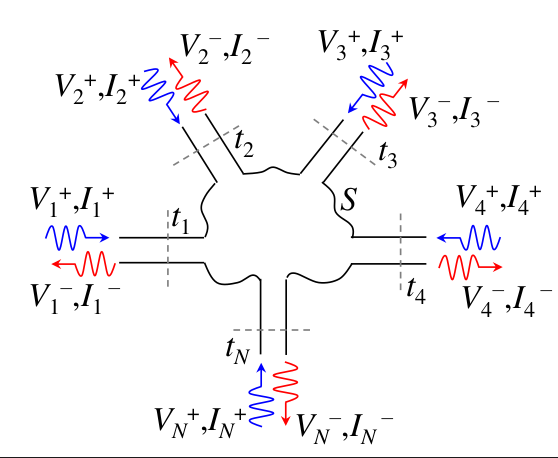
\includegraphics[height=7cm]{imRedeuOndas.png}
	\legend{Fonte: ver \cite{ribeiro}.}
\end{center}

A matriz de impedância $\left[Z\right]$ relaciona as tensões e
correntes, por
\begin{equation*}
	Z_{ij}=\ddfrac{V_i}{I_j}|_{I_k=0\text{ para }k\neq j}
\end{equation*}


$Z_{ij}$ pode ser
encontrado alimentando a porta $j$ com a corrente $I_j$, $V_1^-$,$I_1^-$
abrindo o circuito de todas as outras portas (então
$I_k = 0A$ para $k \neq j$, onde $k$ representam as outras
portas) e medindo a tensão de circuito aberto na
porta $i$.


A matriz de admitância $\left[Y\right]$ é definida como
\begin{equation*}
	\left[Y\right]=\left[Z\right]^{-1}
\end{equation*}
com seus termos dadas por
\begin{equation*}
	Y_{ij}=\ddfrac{I_i}{V_j}|_{V_k=0\text{ para }k\neq j}
\end{equation*}


$Y_{ij}$ pode ser encontrado alimentando a porta $j$ com a tensão $V_j$ , medindo a corrente do
circuito na porta $i$ para todas as outras portas em curto-circuito (então $V_k = 0V$ para $k \neq j$).


Uma rede recíproca apresenta nenhum dispositivo ativo ou meio não
recíproco, como ferritas ou plasmas. Neste tipo de rede, 
matrizes de impedância e admitância são
simétricas, ou seja, $Z_{ij}=Z_{ji}$ e $Y_{ij}=Y_{ji}$, consequentemente, $\left[Z\right]=\left[Z\right]^t$ e $\left[Y\right]=\left[Y\right]^t$.



	% ----------------------------------------------------
% Referências bibliográficas
\makeatletter
\renewcommand\@biblabel[1]{{\parbox{0.8cm}{[#1]}}} %??
\makeatother
\bibliography{bibliografia}         %??
% ----------------------------------------------------
\end{document}